\chapter{Numerical Experiments}
\label{ch:numeric}

%The ESI methods described in Chapter \ref{ch:review} are tested using synthetic data and evaluated using the metrics defined in the same chapter.

Following the model equation from the forward model,
$\Y = \G \SA + \varepsilon$,
each trial of synthetic data is constructed following these steps:
\begin{enumerate}
    \item Construct the leadfield matrix $\G$ based on pertinent anatomical data.
    \item Select a `seed' dipole at random to determine the location of the source patch.
    \item Construct the source distribution, $\SA$, based on the source patch.
    \item Construct a noiseless version of the EEG measurements, $\Y_0 = \G \SA$.
    \item Construct some additive noise, $\varepsilon$, in order to achieve a prescribed Signal-to-Noise Ratio $\ppar{\text{SNR}_\text{dB}}$ measured in decibels.
    \item Construct the EEG measurements, $\Y = \Y_0 + \varepsilon$.
\end{enumerate}

After each trial of synthetic data is created, ESI is performed to estimate the source distribution by using some of the methods described in Chapter \ref{ch:review}.
%
The performance of these methods is then measured using the performance metrics described in the same chapter.

It is important to mention that whenever an ESI method depended on a parameter, its value was determined using either Generalized Cross-Validation (GCV) or U-curve criterion when GCV was not possible.

\section{Forward Model}

For the construction of synthetic data, anatomy data was taken from the ICBM 152 template \cite{icbm152_2011}. 
%
%As the name suggests, the ICBM152 template was constructed as an `average' T1 MRI scan from 152 subjects.
%
Segmentation and surface extraction were omitted since these surfaces are provided with the template.
%
These surfaces are displayed in figure \ref{fig:surfaces}.

\begin{figure}
\centering
%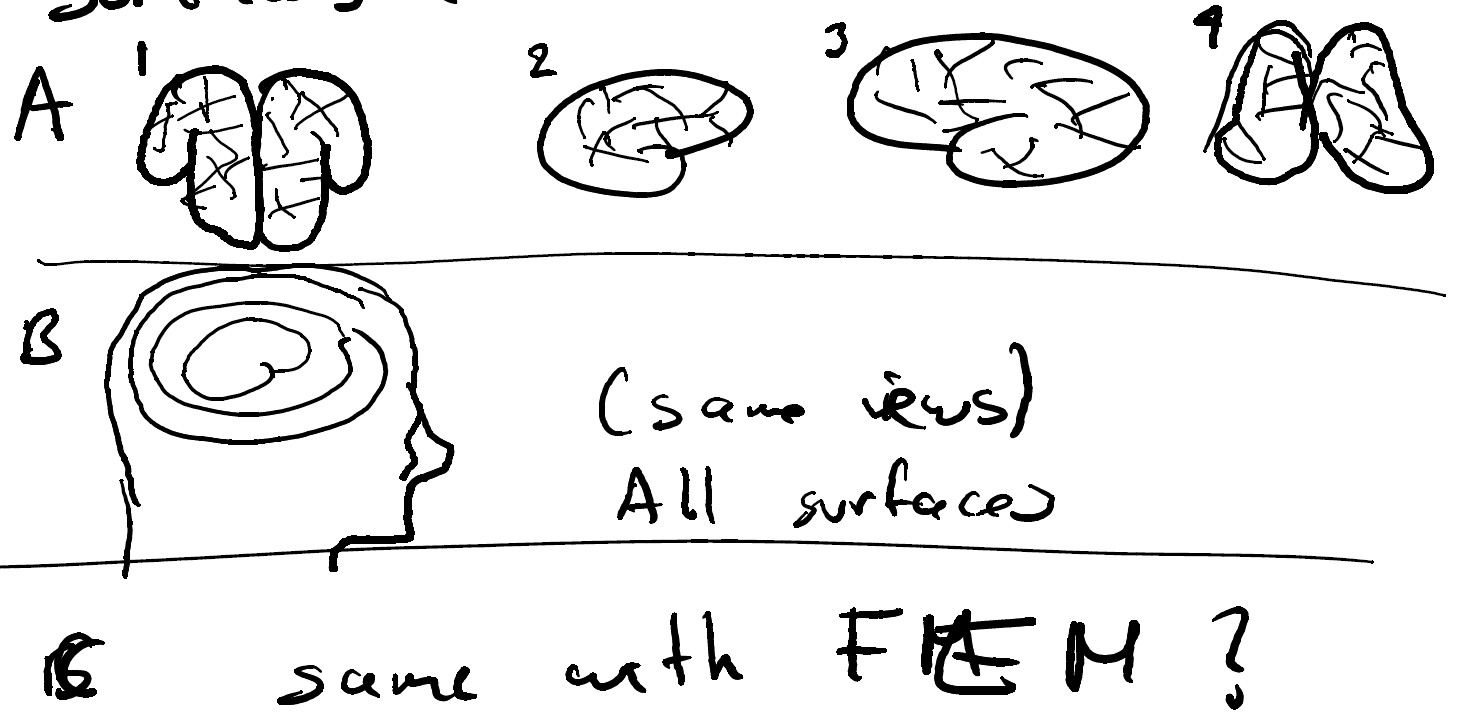
\includegraphics[width=0.8\linewidth]{./img_dev/nsSetupForward}
%
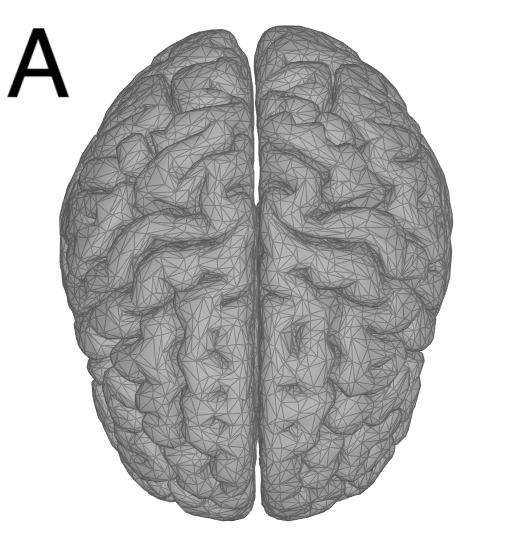
\includegraphics[width=0.18\linewidth]{./img_dev/3D_Subject_ICBM152_2019b_top - Copy2}
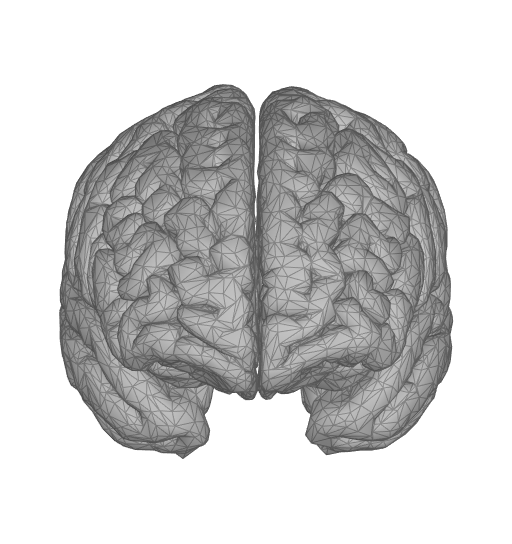
\includegraphics[width=0.18\linewidth]{./img_dev/3D_Subject_ICBM152_2019b_front}
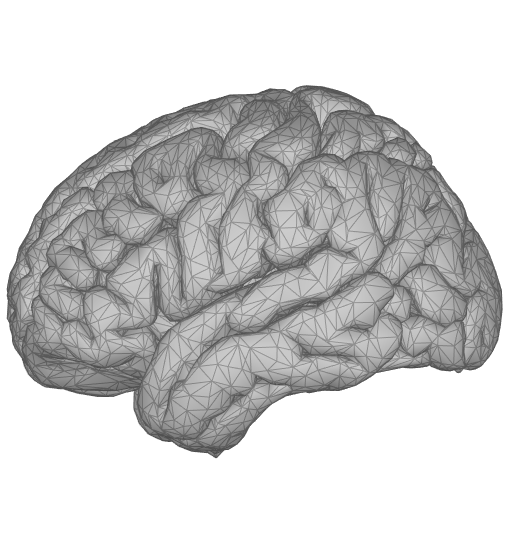
\includegraphics[width=0.18\linewidth]{./img_dev/3D_Subject_ICBM152_2019b_left}
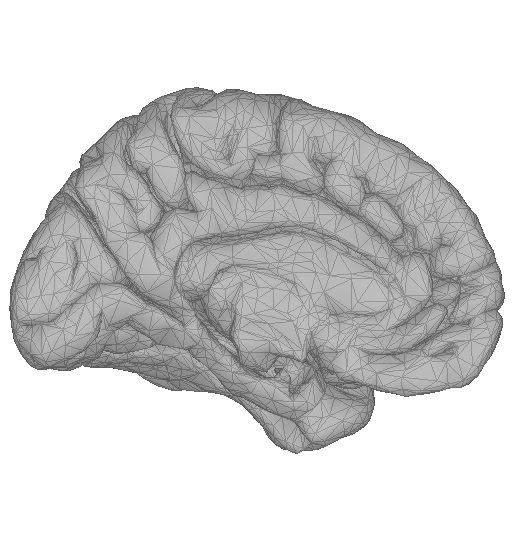
\includegraphics[width=0.18\linewidth]{./img_dev/3D_Subject_ICBM152_2019b_left_inner}
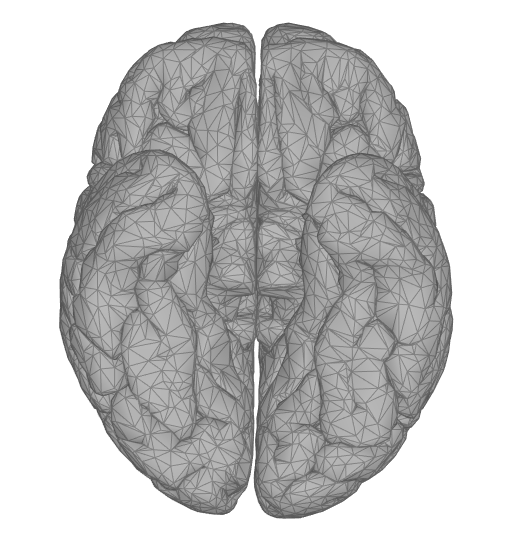
\includegraphics[width=0.18\linewidth]{./img_dev/3D_Subject_ICBM152_2019b_bottom}
%
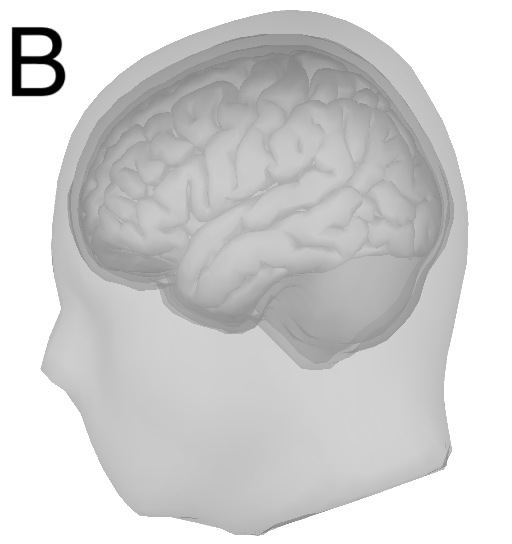
\includegraphics[width=0.2\linewidth]{./img_dev/combined - Copy}
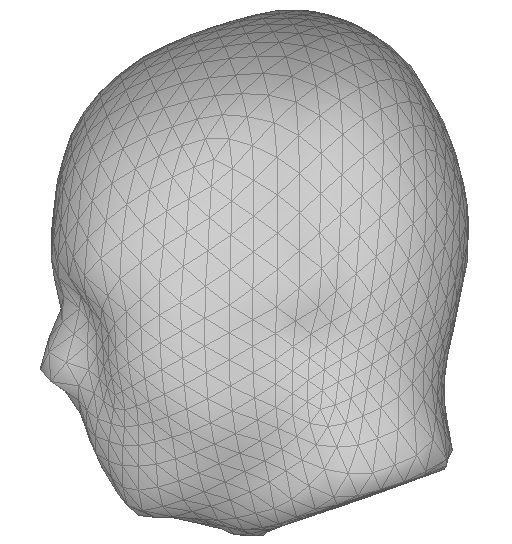
\includegraphics[width=0.18\linewidth]{./img_dev/combined_scalp}
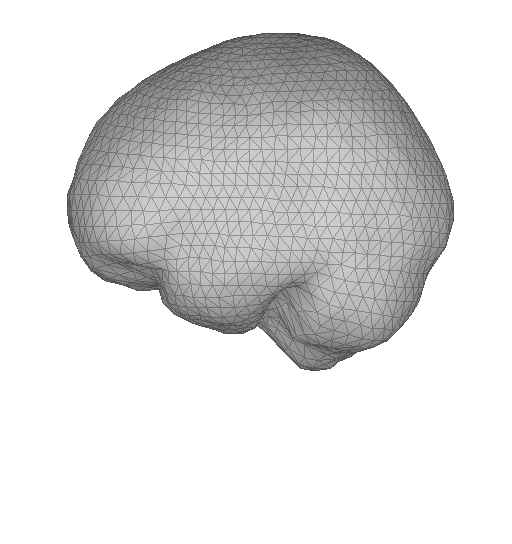
\includegraphics[width=0.18\linewidth]{./img_dev/combined_skull_outer}
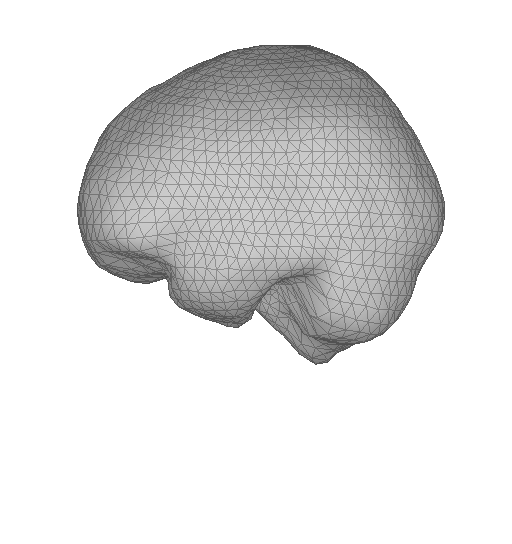
\includegraphics[width=0.18\linewidth]{./img_dev/combined_skull_inner}
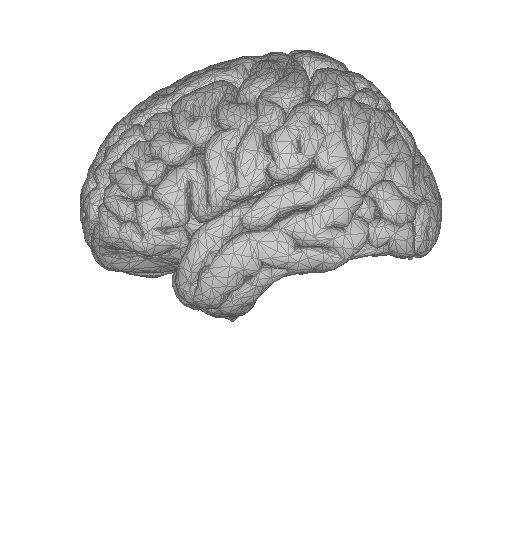
\includegraphics[width=0.18\linewidth]{./img_dev/combined_cortex}
\caption{A. Cortex surface for the ICBM 152 template, consisting of 15,002 vertices. Views from top, left, right, back. B. Triangulated surfaces used for the 4-sphere forward model: cortex, inner skull, outer skull, head}
\label{fig:surfaces}
\end{figure}

Electrodes were placed according to the 10-10 International System; a total of $M=90$ electrodes were considered. 
%
See either figure \ref{fig:1010system} for visual reference or \cite{1020comparison} for a more precise description of the electrode placement protocol.
%
No reference electrode is considered for the synthetic data; the sensor data will be re-referenced to the average.

The positions of the distributed dipoles were set along the brain cortex, and their orientation was orthogonal to the cortex.
%
A total of $N=15,002$ electrodes were considered.

For illustrative purposes, the duration of the recordings was set to a total of $T=1$ time stamps.

\begin{figure}
\centering
%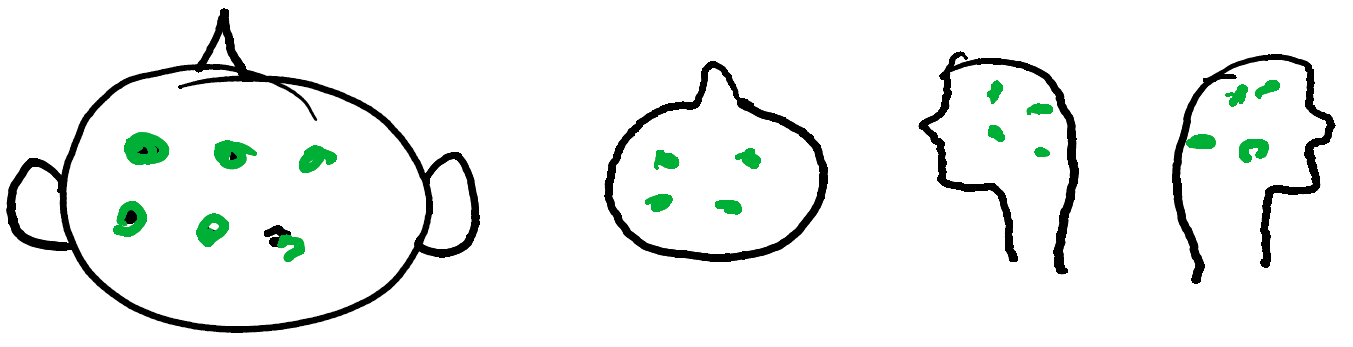
\includegraphics[width=0.8\linewidth]{./img_dev/nsElectrodeSetup}
\includegraphics{./img/EEG_10-10.pdf}
%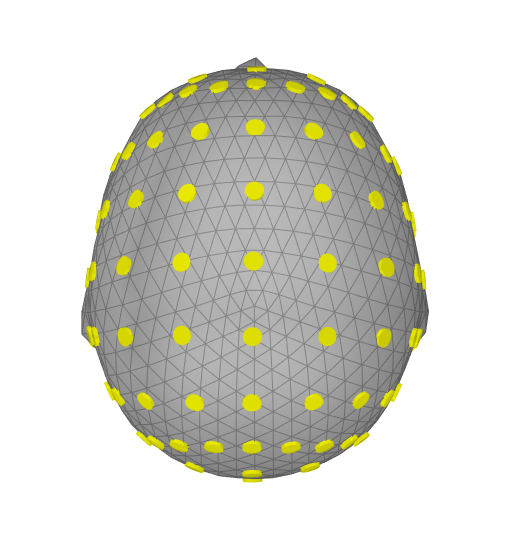
\includegraphics[width=0.25\linewidth]{./img_dev/EEG_3D_Subject_ICBM152_2019b_top}
%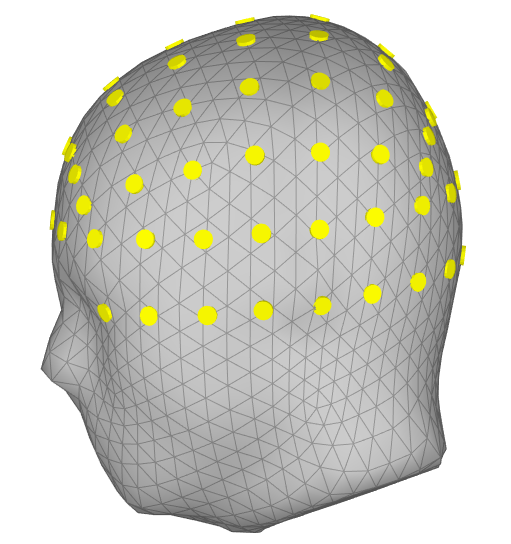
\includegraphics[width=0.25\linewidth]{./img_dev/EEG_3D_Subject_ICBM152_2019b_left}
%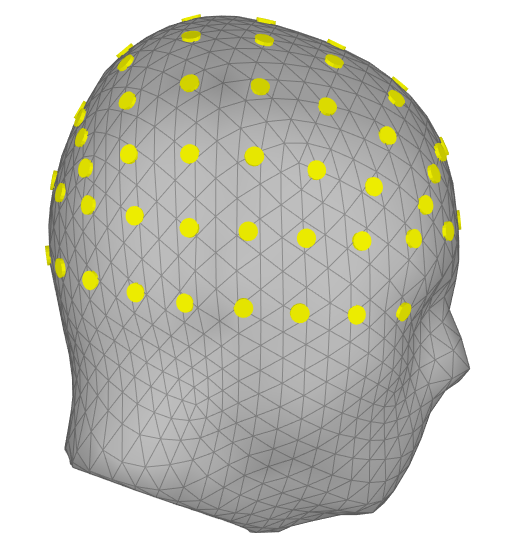
\includegraphics[width=0.25\linewidth]{./img_dev/EEG_3D_Subject_ICBM152_2019b_right}
\caption{Electrode Placement according to the 10-10 International System. A. Schematic with the electrode labels. B. Electrodes at the ICBM152 template head}
\label{fig:1010system}
\end{figure}

%\subsubsection{Synthetic data protocol}

\subsection{Source Distribution}

The source distribution, $\SA$, is constructed by considering one small source patch; the dipoles in the source patch are selected as those being close to a seed dipole, indexed by $n^*$.
%
The seed dipole was selected randomly for each trial; a total of 30 trials were simulated.

After selecting the seed dipole, indexed by $n^*$, $\SA$ is constructed as
\begin{equation}
\SA(n) = f\ppar{ \nnorm{\rr_n-\rr_{n^*}} / \kappa }
\end{equation}
with $\rr_n$ the location of the $n$-t dipole, $f:\R_+\rightarrow \R$ a decreasing function, and $\kappa>0$ a scaling parameters.

For illustrative purposes, four different options for $f$ are considered:
\begin{align}
\text{Square} &&
    f_\text{sq}(x) 
    &= 
    \begin{cases}
1, &\text{if } x\leq 1 \\
0, &\text{otherwise}.
\end{cases}
    \\
\text{Gaussian} &&
    f_\text{Gauss}(x) 
    &= 
    e^{-x^2/\kappa}
    \\
\text{Exponential} &&
    f_\text{exp}(x) 
    &= 
    e^{-x/\kappa}
    \\
\text{Polynomial} &&
    f_\text{pol}(x) 
    &= 
    \sqrt{ \max\,\, \sset{1-\ppar{\frac{x}{\kappa}}^2, 0 }}
\end{align}

%The selection of these functions follows a survey of the literature.
%
Apart from point sources, source patches created using $f_\text{sq}$ are fairly common; their sharp edges facilitate determining the size of the source patch without ambiguity.
%
Some other papers have used $f_\text{Gauss}$ to obtain source patches that are smooth in space. 

Functions $f_\text{exp}$ and $f_\text{pol}$ are introduced here to produce source patches with intermediate properties.
%
The source patches constructed using $f_\text{pol}$ have a finite support and a smooth peak, while the ones built using $f_\text{exp}$ present spatial smoothness, a sharp peak, and a `heavy tail' in space.
%
See figure \ref{fig:exaple_true} for a visual example of these properties.

\begin{figure}
\centering
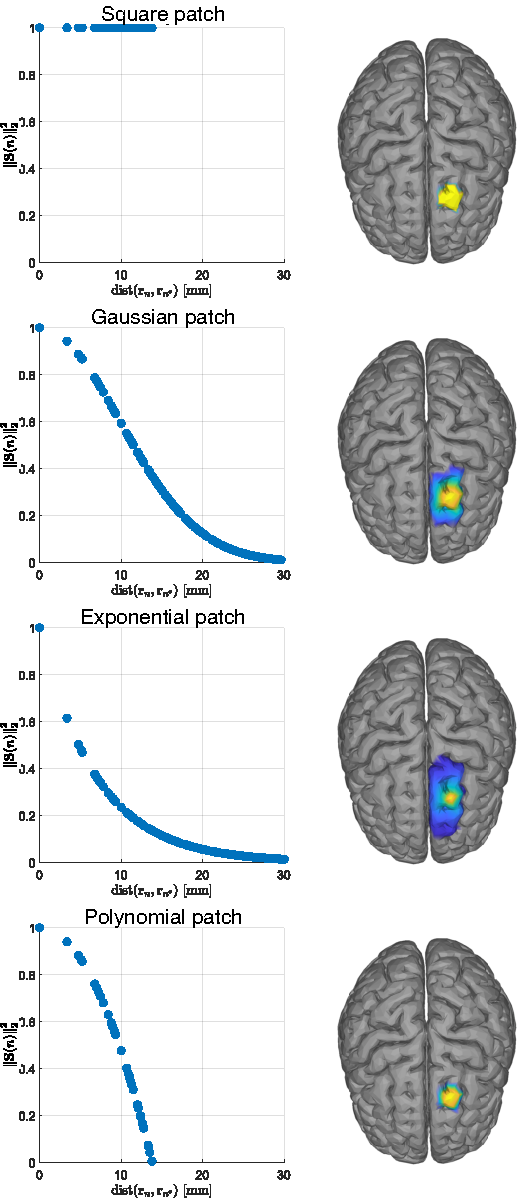
\includegraphics[scale=0.9]{./img/profiles.pdf}
\caption{Different source patches used to generate synthetic data}
\label{fig:exaple_true}
\end{figure}

%This type of configuration is referred to as `source patches' or `extended sources' since it occupies an area too large to be modeled as a single dipole.

For the synthetic data in this chapter, we set $\kappa = $ 12.6 \si{mm} in order to obtain source patches with a surface area of approximately 5 \si{cm^2}.

\subsection{Noise}

For simplicity, only additive white noise is added to the sensors, i.e. we use 
\begin{equation}
    \varepsilon(t,:) \sim \nnorm{0, \diag{\sigma_1, \dots, \sigma_M}^2}
\end{equation}
with $\sigma_m \geq 0$ for $m=1, \dots, M$ the noise variances for each EEG electrode.

%within the model formulation, we considered no internal noise ($\nu=0$) and independent Gaussian noise at the sensors, i.e. $\varepsilon_m \sim\norm\ppar{0, \sigma_m^2}$ for $m = 1, \dots, M$ for some parameters $\sigma_m\geq 0$.
%
Under these conditions the noisy recordings, $\Y$, have the following distribution
\begin{equation}
\ppar{\Y \given \SA} =
\norm\ppar{ \G\, \SA, \diag{\sigma_1, \dots, \sigma_M}^2 }
\end{equation}

The channel SNR (in decibels) for the $m$-th sensor is given by
\begin{equation}
\text{SNR}_m = 
10\, \log_{10}\ppar{ \frac{ \ppar{ \spar{\G\, \SA}(m)}^2 }{\sigma_m^2} }
\end{equation}
With a prescribed SNR value, the parameters $\sigma_m$ are selected as follows
\begin{equation}
\sigma_m^2 = 
10^{{-{SNR}/{10}} }
\spar{\G\, \SA}(m)
\end{equation}

Based on informal observations, we consider that an SNR level of 20 dB is a low-noise condition.
%
Notice that the condition of lack of noise is attached to $\sigma_m = 0$ and $\text{SNR} = \infty$.

%%%%%%%%%%%%%%%%%%%%%%%%%%%%%%%%%%%%%%%%%%%%%%%%%%%%%%%%
%%%%%%%%%%%%%%%%%%%%%%%%%%%%%%%%%%%%%%%%%%%%%%%%%%%%%%%%

%\section{Multi-modal asymmetric methods}
%
%A common framework
%to enhance ESI is to incorporate 
%`information' from the additional {modalities} of data:
%%and then constrain ESI to it.
%%
%%Multiple authors have explored the idea 
%%of enhancing 
%%the EEG Source Localization
%%by adding data from other `modes' of data: 
%MEG, MRI/fMRI\cite{he2008multimodal, huster2012methods}, PET, fNIRS\cite{fnirs}, etc.
%(Figure based on \cite{he2008multimodal}).
%%of using additional data to aid the EEG Source Localization, would it be MEG.
%\begin{figure}
%\centering
%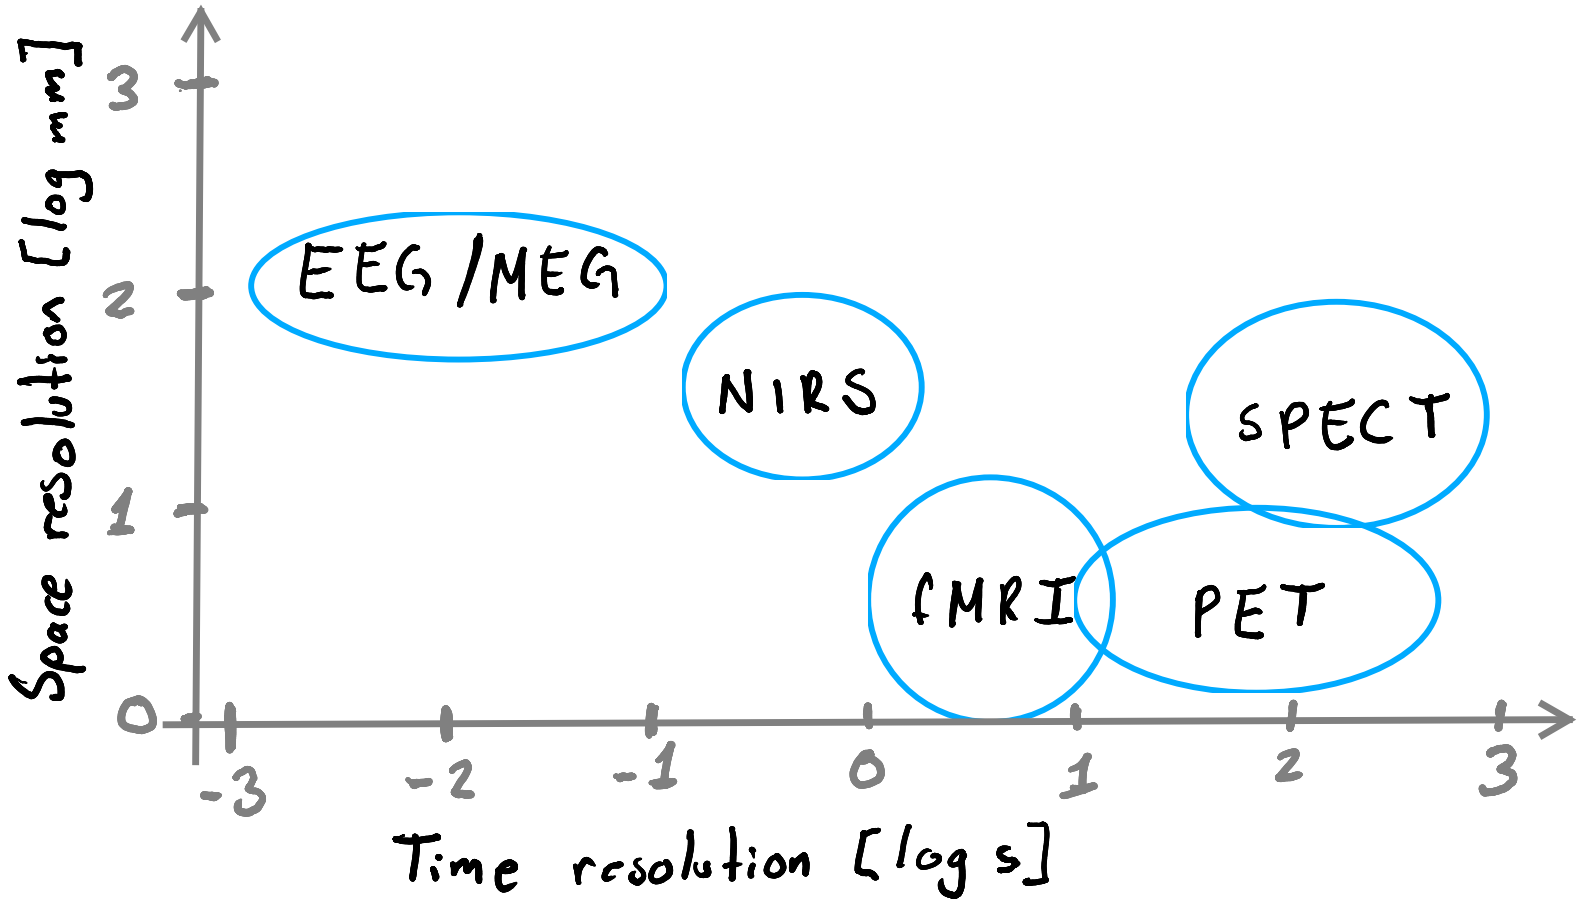
\includegraphics[width=0.65\linewidth]{./img_final/sketch07}
%\caption{PET=Positron Emission Tomography, NIRS=Near Infrared Spectroscopy, SPECT=Single-Photon Emission Computed Tomography}
%\end{figure}
%
%
%One big conceptual challenge for multimodal data integration is to model the interaction of the underlying physical phenomena. 
%%
%Focusing only on unilateral interactions results in asymmetric data integration.
%
%%For
%%asymmetric data integration, 
%%such as enhanced ESI, 
%%some bilateral interactions may be simplified. 
%%Thus 
%
%{Asymmetric data fusion} is the extraction of some parameters from one modality, which then are used to further the  for ESIanalysis of the other modaliFor ESI, the obtained parameters are typically used within the penalty functions.
%%Some simplifying assumptions considered in the literature for asymmetric data fusion for ESI are:
%%A common framework
%%Some techniques used in the literature 
%%to ESI enhancing is to extract `information' from the additional modalities and then constrain ESI to it.
%Some of the parameters extracted include:
%\begin{itemize}
%    \item Correlation networks
%    \item Statistical Parametric Maps (SPM)
%    \item Hidden activation variables \cite{fire}
%\end{itemize}

